\section{HODMD Analysis of the NH$_3$/H$_2$ Non-Premixed Reacting Mixing Layer}
\label{sec:coria}

\subsection{NH$_3$/H$_2$ non-premixed mixing layer}
\label{sec:DATA_CORIA}

This dataset consists of direct numerical simulations (DNS) of a two-dimensional non-premixed ammonia-hydrogen-air reacting mixing layer. It is generated by DCGIOVANNI at CORIA using the structured mesh reactive flow solver SiTCom-B \cite{sitcomb}. The configuration represents a splitter-plate stabilized flame in which a cold fuel stream and a hot air stream interact across a shear layer, representative of conditions encountered in practical burners.

The lower stream consists of a NH$_3$/H$_2$ fuel blend (with 15\% H$_2$ by volume) at ambient temperature (300~K) with a mean velocity of 15~m~s$^{-1}$, while the upper stream consists of preheated air with a mean velocity of 39.6~m~s$^{-1}$. A cold wall maintained at 600~K is imposed at the top boundary, and a symmetry condition is applied at the bottom. Homogeneous velocity fluctuations of 10\% are prescribed at both inlets. The computational domain measures $12 \times 1$~cm and is discretized on a uniform grid of $2400 \times 200$ cells with a resolution of 50~$\mu$m.

\FloatBarrier
\begin{figure}[htbp]
    \centering
    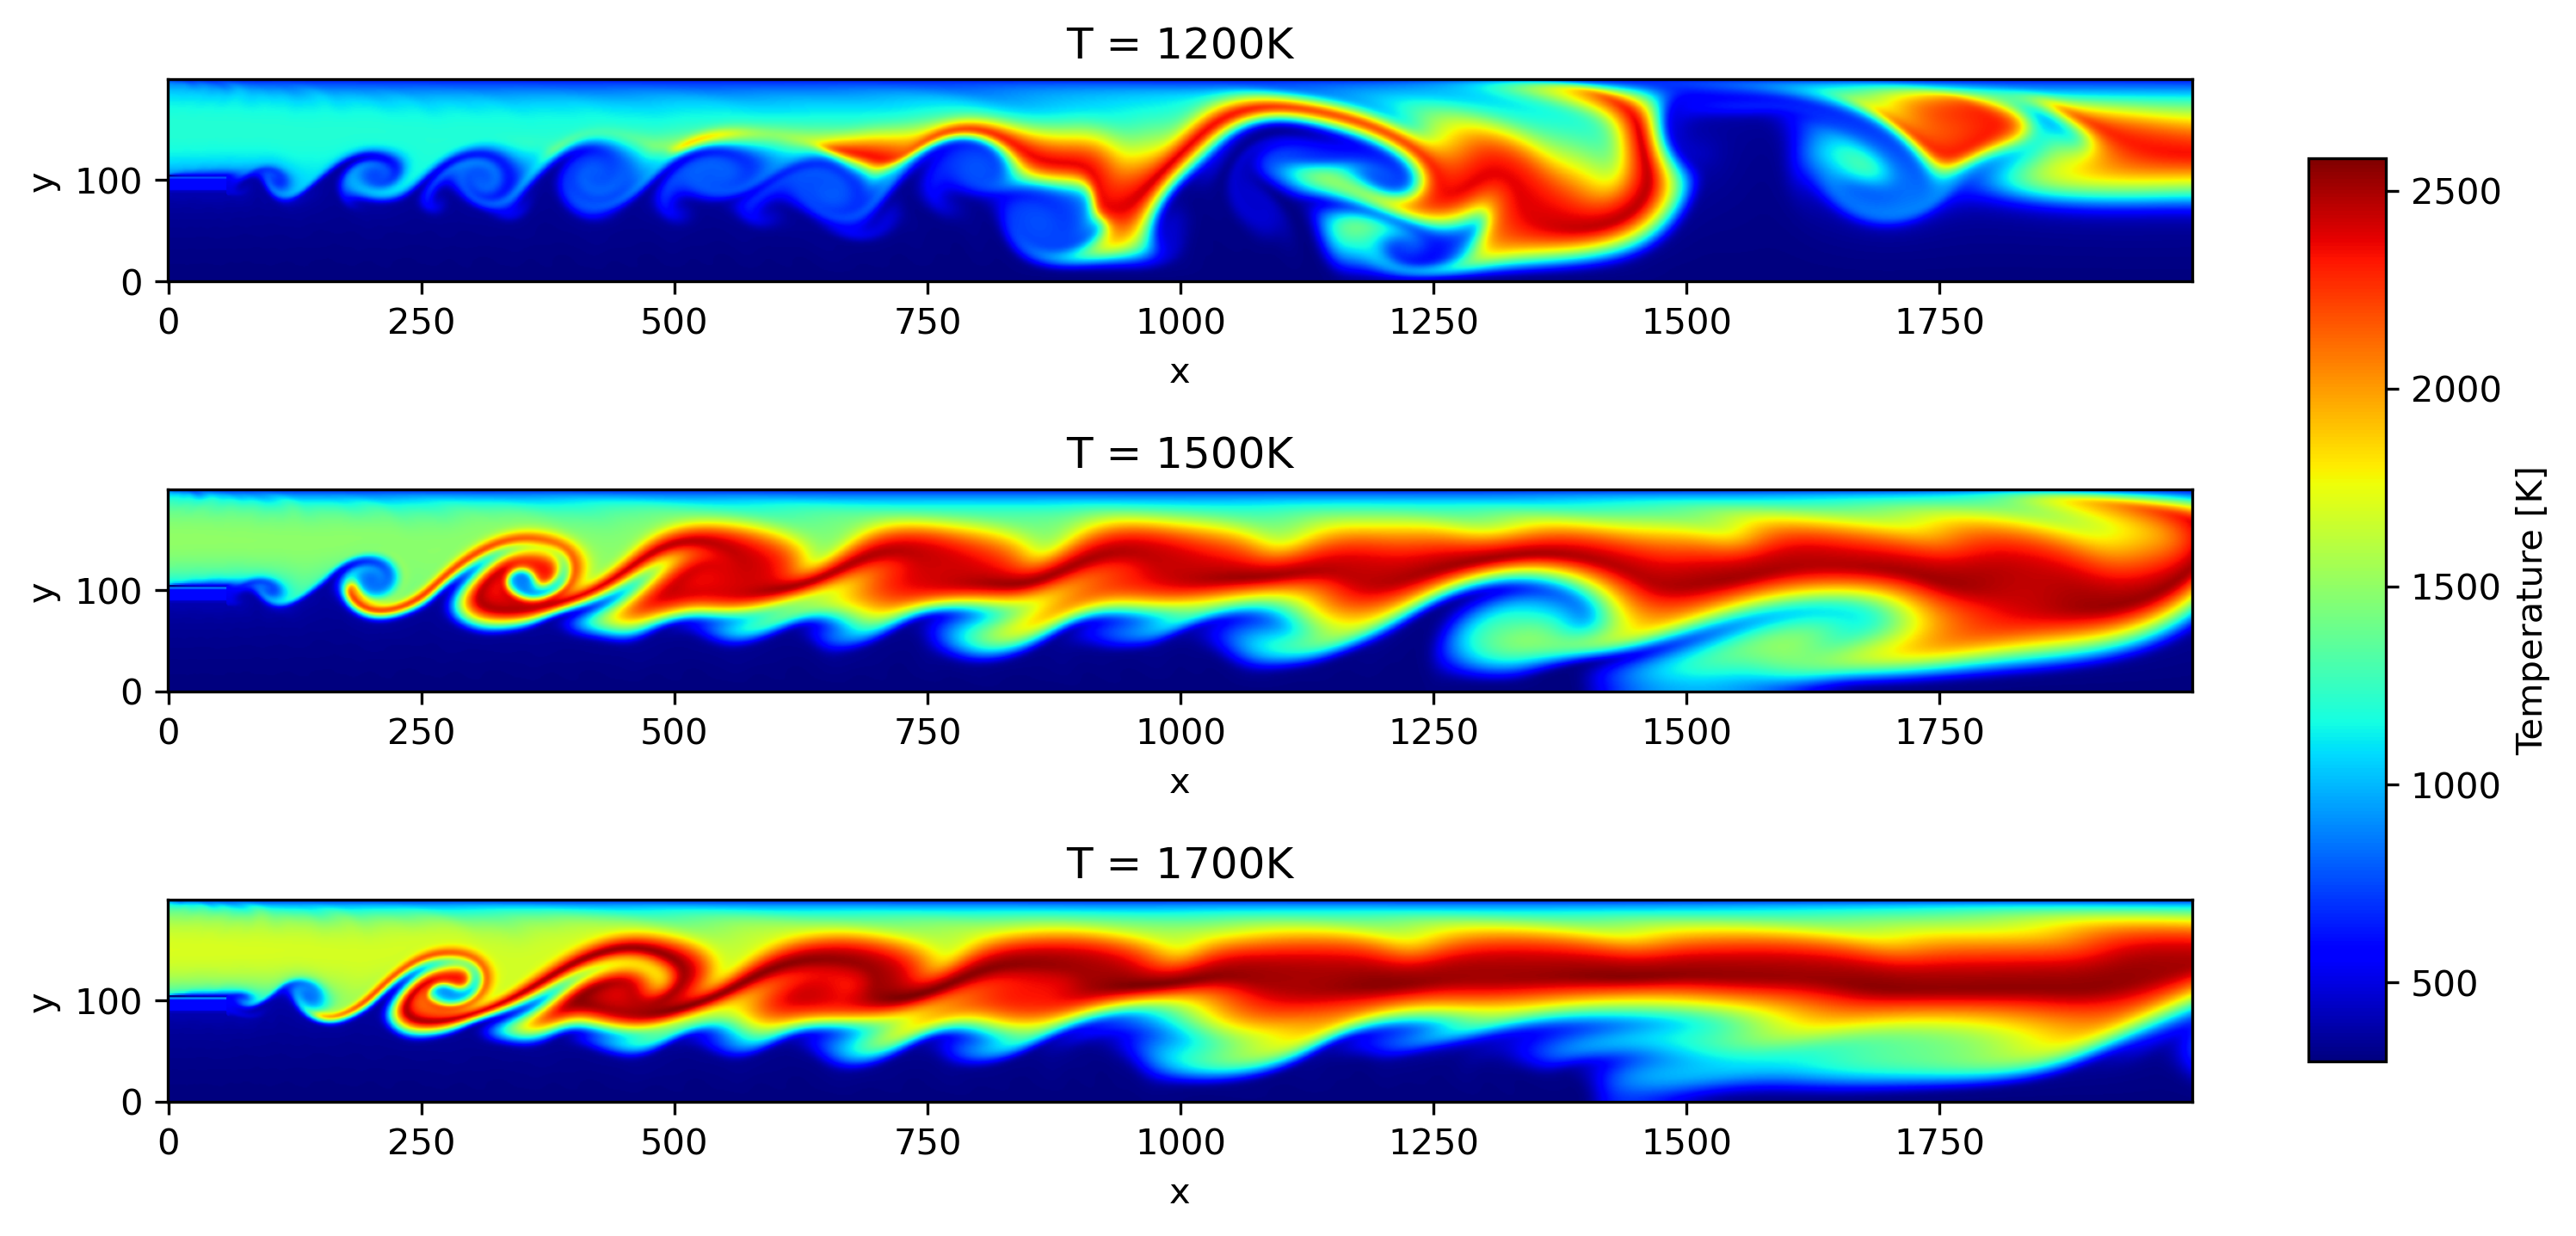
\includegraphics[width=0.85\textwidth]{../IMAGES/DATASETS/coria_3snap.png}
    \caption{Three representative snapshots of the temperature field from the NH$_3$/H$_2$ non-premixed reacting mixing layer DNS, illustrating the spatial evolution of the flame and mixing structures at different instants.}
    \label{fig:coria_data}
\end{figure}
\FloatBarrier

Three datasets are generated at different air preheat temperatures, namely 1200~K, 1500~K, and 1700~K, to probe the sensitivity of the flame dynamics and species evolution to the inlet thermal boundary condition. The domain geometry, grid resolution, and flow velocities are identical across all three cases. Each snapshot contains 19 reactive scalar fields corresponding to the species of the reduced mechanisms RmAH-1 and RmAH-2 \cite{grassi2025} — namely H$_2$, O$_2$, H$_2$O, H, O, OH, HO$_2$, NH$_3$, NH$_2$, NH, N, NO, NO$_2$, N$_2$O, HNO, NNH, N$_2$H$_2$, N$_2$, and Ar — together with temperature, yielding 20 variables in total. The species analysis presented in this work is conducted exclusively on the 1500~K dataset, which constitutes the reference operating condition for the assessment of the proposed methodologies.

\subsection{Methods}
\label{sec:methods_coria}

\subsubsection{High Order Dynamic Mode Decomposition}
\label{sec:dmd_hodmd}

Dynamic Mode Decomposition (DMD)~\cite{schmid2010}  is a data-driven spectral method that extracts spatially coherent structures and their associated temporal dynamics directly from time-resolved snapshot~\footnote{Matrix that has as columns (rows) the time index and all the other unfolded indices as rows (columns)} data.
Given a sequence of snapshots $\mathbf{v}_k \in \mathbb{R}^{J}$, $k = 1,\dots,K$, DMD seeks a linear operator $\mathbf{A}$ such that $\mathbf{v}_{k+1} \approx \mathbf{A}\,\mathbf{v}_k$, whose leading eigenpairs encode the dominant frequencies and growth/decay rates of the system.
The full data field is then expressed as a superposition of DMD spatial modes $u_p(\mathbf{x})$ with purely exponential temporal evolution,
\begin{equation}
    v(\mathbf{x},t) = \sum_{p=1}^{P} a_p\, u_p(\mathbf{x})\, e^{(\delta_p + i\omega_p)(t-1)\Delta t},
    \label{eq:dmd_expansion}
\end{equation}
where $a_p \geq 0$ are real amplitudes, $\omega_p$ are angular frequencies, $\delta_p$ are growth rates, and $\Delta t$ is the sampling interval.
Each mode is normalised so that its root-mean-square norm equals unity.

Higher-Order Dynamic Mode Decomposition (HODMD)~\cite{leclainche2017} extends DMD making it more suitable for noisy data and nonlinear phoenomena such as the ones ecnountered dealing with combustion data. The main idea is to extend the assumption that the system's evolution can be described with a linear operator to temporal windows of size $d$. Each snapshot is thus related to the $d$ subsequent snapshots through a set of linear operators.
This generalised assumption leads to a sliding-window construction of an augmented snapshot matrix and allows for better identification of close frequency even in noisy data. When $d = 1$, HODMD reduces exactly to standard DMD.

The HODMD algorithm proceeds in two main steps:\\
\emph{Step~1 — Dimensionality reduction via SVD.}\label{subsec:svd_dmd}
A truncated Singular Value Decomposition (SVD) is applied to the original snapshot matrix, compressing the spatial dimension from $J$ to $N$ retained singular values.
The tolerance $\varepsilon_{\mathrm{SVD}}$ controls the level of compression by enforcing
\begin{equation}
    \frac{\sigma_j}{\sigma_1} \geq \varepsilon_{\mathrm{SVD}},
    \label{eq:svd_trunc}
\end{equation}
where $\sigma_j$ are the singular values in decreasing order.
The resulting temporal coefficients weighted by the retained singular values form the reduced snapshot matrix, which filters noise.\\
\emph{Step~2 — High-order Koopman eigenvalue problem.}
HODMD is applied to the reduced snapshot matrix with delay parameter $d$.
The eigenvalue problem is solved to extract DMD modes, frequencies and amplitudes.
A second tolerance $\varepsilon_{\mathrm{DMD}}$ selects physically significant modes by retaining only those whose relative amplitude satisfies
\begin{equation}
    \frac{a_p}{\max_p(a_p)} > \varepsilon_{\mathrm{DMD}}.
    \label{eq:dmd_trunc}
\end{equation}

\paragraph{Physical interpretation}

From a practical point of view DMD looks for coherent structures that behave in an oscillatory manner across the whole dataset. This makes it easier to observe phonomena that cannot be observed when looking at the original data, that often is very complex. A big issue is that the assumption that the system can be described with a matrix even in snapshot form is very strong and it will fail in case of noisy or turbulent data.
HODMD is able to obtain better results because instead of looking for oscillatory coherent structures across the whole dataset, it looks for structures that depend on the last d snapshots instead of just the last one. This makes it possible to extract up to $d \times N$  modes instead of N:
\begin{equation*}
\underbrace{\mathbf{v}_{k+1} = \mathbf{A}\,\mathbf{v}_k}_{\text{DMD}}
\quad \longrightarrow \quad
\underbrace{\mathbf{v}_{k+d} = \mathbf{A}_1\,\mathbf{v}_{k+d-1} + \mathbf{A}_2\,\mathbf{v}_{k+d-2} + \cdots + \mathbf{A}_d\,\mathbf{v}_k}_{\text{HODMD}}
\end{equation*}

\subsubsection{Multidimensional Iterative HODMD (mdHODMDit)}
\label{sec:method_mdhodmd}

\paragraph{High Order Singular Value Decompostion}

Both DMD and HODMD perform truncated SVD for denoising and dimensionality reduction. This effectively filters out structures that have very low temporal contribution across the whole dataset, which often coincides with noise. Combustion data often carry several physical variables and span a multi-dimensional spatial domain. The application of SVD on the reshaped tensor introduces an implicit coupling among modes that belong to different dimensions, and the SVD truncation cannot distinguish noise contributions arising from the spatial, temporal, or variable axes independently.
For this reason, a first improvement over the classical version of HODMD is to introduce High Order Singular Value Decomposition (HOSVD) \cite{de2000multilinear} in the first step. This is a generalization of SVD that allows filtering along each dimension of the tensor.

It works on data keeping it in tensor form $\mathcal{T} \in \mathbb{R}^{N_{\mathrm{var}} \times N_x \times N_y \times N_t}$.
First, it unfolds $\mathcal{T}$ along each of its four modes in turn, computes the
$n$-mode singular values $\{\sigma_j^{(n)}\}$ from the corresponding unfolded matrix, and
retains factor matrices $\mathbf{U}^{(n)}$ by enforcing the truncation criterion
\begin{equation}
    \frac{\sigma_j^{(n)}}{\sigma_1^{(n)}} \geq \varepsilon_{\mathrm{tol}},
    \label{eq:hosvd_trunc}
\end{equation}
independently for each mode $n$.
The result is a compressed core tensor $\mathcal{S}$ and a set of factor matrices
$\{\mathbf{U}^{(n)}\}_{n=1}^{4}$ such that
$\mathcal{T} \approx \mathcal{S} \times_1 \mathbf{U}^{(1)} \times_2 \mathbf{U}^{(2)}
\times_3 \mathbf{U}^{(3)} \times_4 \mathbf{U}^{(4)}$,
where $\times_n$ denotes the $n$-mode product. These matrices are exactly the ones one would obtain performing truncated SVD on each of the unfodlings.
Therefore, the temporal factor matrix $\mathbf{U}^{(4)}$ is the same as before.

\FloatBarrier
\begin{figure}[htbp]
    \centering
    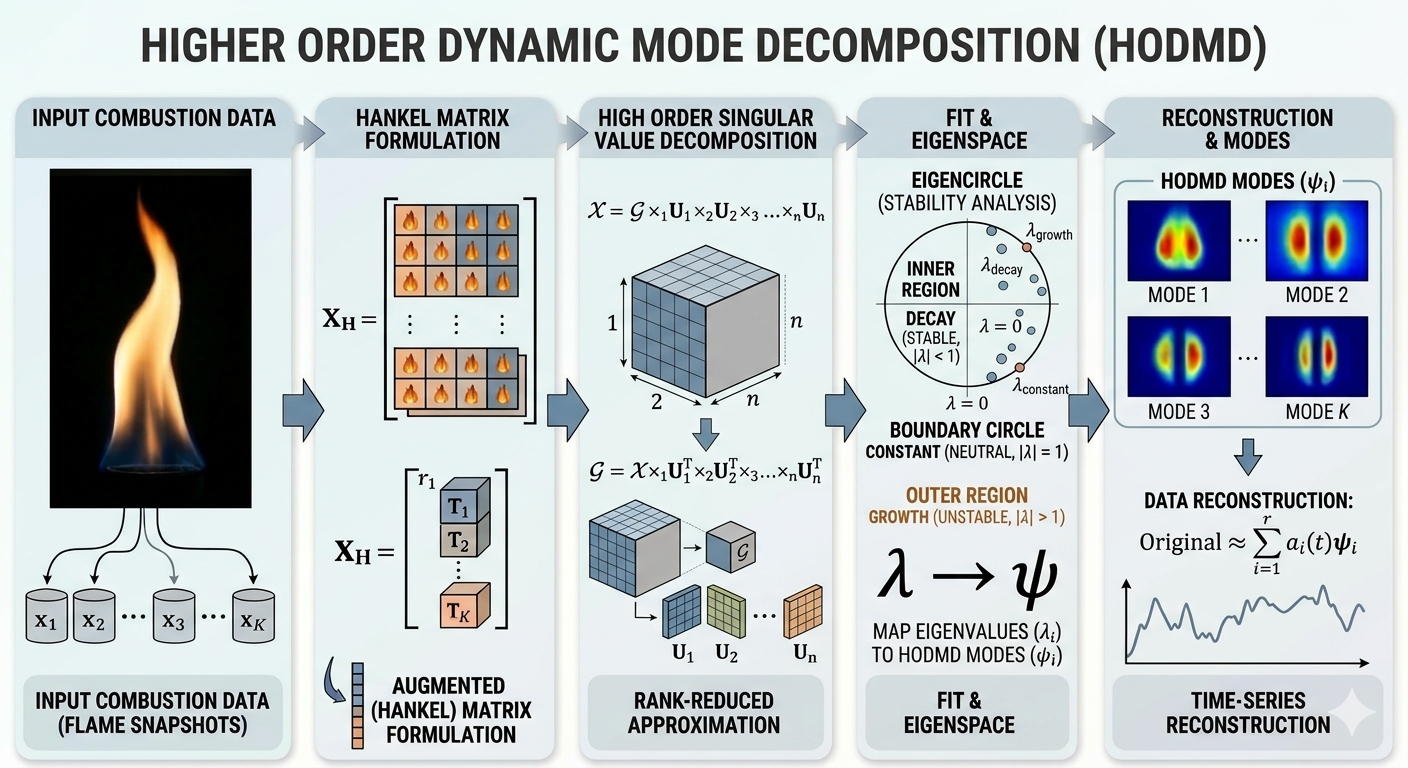
\includegraphics[width=0.85\textwidth]{../IMAGES/HODMD.png}
    \caption{Scheme rapresenting High Order Dynamic Mode Decomposition on combustion data}
    \label{fig:hodmd}
\end{figure}
\FloatBarrier

After the DMD eigendecomposition,the reduced spatial DMD modes are projected back to the original tensor dimensions by contracting with the spatial
factor matrices $\mathbf{U}^{(1)}, \mathbf{U}^{(2)}, \mathbf{U}^{(3)}$ and the core tensor, recovering physically interpretable spatial structures in the full variable-$x$-$y$ space without ever vectorising the multi-variable field, from this the algorithm is called mutlidimensional.

Then, the procedure is iterated. The DMD reconstruction is used to form an updated snapshot tensor, which is re-compressed via HOSVD. The spatial ranks $r_x$, $r_y$, and $r_{\mathrm{var}}$ retained after truncation are monitored: if they
differ from those of the previous iteration, the HODMD step is repeated on the new compressed temporal matrix $\hat{V}_1^K$. Convergence is declared when the spatial ranks no longer change between two successive iterations. This can be intepreted as the low-rank spatial  structure implied by the DMD modes is the same as the one identified by HOSVD.

\paragraph{Identification of Physical Frequencies}
\label{sec:coria_frequencies}
Once the analysis is calibrated and run for a sufficient number of parameters, one can find physical frequencies and modes. In order to find these modes, one must look at the frequency amplitude spectra, focusing on the peaks, i.e. frequencies. Physical modes should exist regardless of how the observer matrix is built and Therefore be consistent across a wide range of $d$ parameter. Moreover relevant structures should be associated to relevant eigenvectors and not ones close to noise threshold, thus beeing resilient to various tolerance thresholds $\varepsilon_{\mathrm{tol}}$.

\subsection{Results and Discussion}
\label{sec:results_coria}

The main results reported in this section are build upon the work of Pablo López Salazar that first started the collaboration with CORIA. mdHODMDit described in section~\ref{sec:method_mdhodmd} is applied to extract core physical behaviour of the system in the three cases reported in section~\ref{sec:DATA_CORIA}.

\subsubsection{Data Structure and Preprocessing}
\label{sec:coria_preprocessing}

For each case, data is organized in a four dimensional tensor: $\mathcal{T} \in \mathbb{R}^{N_{\mathrm{var}} \times N_x \times N_y \times N_t}$, in which the dimension correspond to variables, the streamwise spatial coordinate $x$, the cross-stream coordinate $y$, and time $t$, respectively.
In order to study the region of physical interest, i.e. the one in which the instability develops and evolves the domain of the streamwise direction is restricted to the range $[0.3, 5.0]$~cm downstream of the splitter plate. This is the near-field flame stabilization region and the initial development of the shear layer. Data was also processed in time discarding the initial transient regime.
For this kind of data, scaling is important due to the differences in the order of magnitude of the variables considered and the differences between their units of measurement \cite{corrochano2023higher, parente2013principal}. Since there is no universally accepted quantitative criterion to determine which scaling method is most appropriate, the analysis was performed using both auto scaling $x_{i}^{\text{scaled}} = \frac{x_i - \mu_x}{\sigma_x}$ and range scaling $x_{i}^{\text{scaled}} = \frac{x_i - x_{\min}}{x_{\max} - x_{\min}}$. The analysis yielded similar results for both scaling methods, identifying the same main frequencies.
For convenience, frequencies are expressed in units of Strouhal number:
\begin{equation}
    St = f \cdot \frac{\ell}{U_b},
\label{eq:strouhal}
\end{equation}
where $\ell = 3$~mm is the reference lenght of the mixing layer and  $U_b$ is the bulk speed, respectively $U_b = 21{,}34$, $24{,}29$ e $27{,}14$~m~s$^{-1}$ for cases at 1200~K, 1500~K e 1700~K.

\subsubsection{Parameter Calibration}
\label{sec:coria_params}

The analysis is performed over a grid of Hankel delay parameters
\begin{equation}
    d \in \{10,\, 15,\, 20,\, 25,\, 30,\, 35,\, 40,\, 45\}
    \label{eq:d_values}
\end{equation}
and tolerance values
\begin{equation}
    \varepsilon_{\mathrm{tol}} \in
    \{5\times10^{-3},\, 2\times10^{-2},\, 3\times10^{-2},\, 4\times10^{-2},\,
      5\times10^{-2},\, 7\times10^{-2},\, 1\times10^{-1},\, 2\times10^{-1}\}.
    \label{eq:tol_values}
\end{equation}
The same tolerance $\varepsilon_{\mathrm{tol}}$ governs both the HOSVD truncation (equation~\eqref{eq:hosvd_trunc}) and the amplitude threshold applied to retain DMD modes.

\subsubsection{Frequency--Amplitude Spectra and associated DMD modes}
\label{sec:freq_amplitude}

The frequency--amplitude plots shown in Figures~\ref{fig:spectrum_1200K}, \ref{fig:spectrum_1500K}, and \ref{fig:spectrum_1700K} display, for each temperature case, the normalised DMD mode amplitudes $|\hat{a}_k| / \max_k |\hat{a}_k|$ as a function of Strouhal number $St$. Each marker corresponds to one $(d, \varepsilon_{\mathrm{tol}})$ pair; different colours encode different values of $d$ and different marker styles encode different tolerances. Peaks that persist across all curves can therefore be read off directly as physically robust frequencies. To showcase the coherent structures associated to these freuqencies, temperature is choosen as the rapresentative variable due to the fact that in many cases is a variable of interest for both experimental and theoretical problems. Despite this, coherent structures for every variable can be plotted.

\paragraph{Case 1200~K}
\label{sec:spectrum_1200K}

The spectrum for the 1200~K case, shown in Figure~\ref{fig:spectrum_1200K}, is characterised by a rich distribution of modes spanning a broad Strouhal range up to $St \approx 1.7$. The dominant peak is located at $St \approx 0.42$ and is reproduced consistently across all $(d, \varepsilon_{\mathrm{tol}})$ combinations, confirming its physical robustness. Secondary peaks of significant amplitude are identified at $St \approx 0.84$, $St \approx 1.26$, $St \approx 1.68$. These peaks are approximately integer multiples of the dominant frequency and therefore interpretable as higher harmonics of the fundamental shear-layer instability.

\FloatBarrier
\begin{figure}[h!]
    \centering
    
\includegraphics[width=\textwidth]{Frequency_amplitude_plot1200.png}
    \caption{Normalised DMD mode amplitudes as a function of Strouhal number for the 1200~K dataset, for $d \in \{35,40,45\}$ and $\varepsilon_{\mathrm{tol}} \in \{5\times10^{-2},\, 7\times10^{-2}\}$.}
    \label{fig:spectrum_1200K}
\end{figure}
\FloatBarrier

The associated modes to the highlighted points in Figure~\ref{fig:spectrum_1200K} are shown in Figure~\ref{fig:modes_1200K}.

\FloatBarrier
\begin{figure}[h!]
    \centering
    \begin{subfigure}[b]{0.48\textwidth}
        \centering
        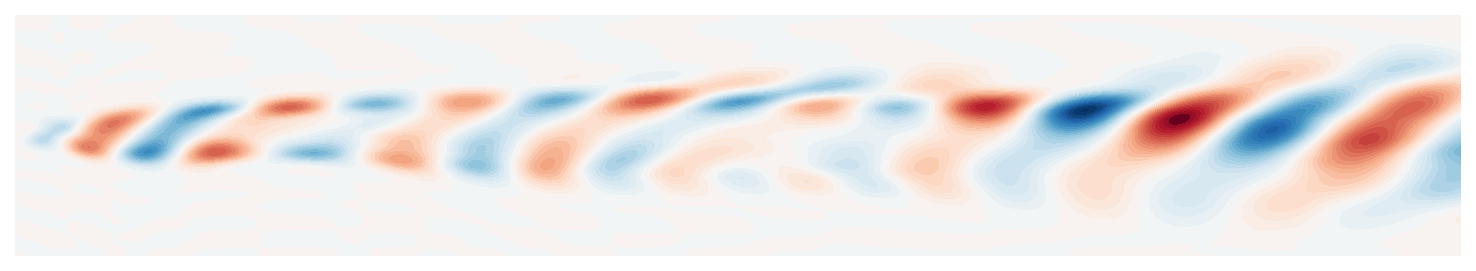
\includegraphics[width=\linewidth]{IMAGES/DMD_MODES_main_freqs_T1200/DMD_mode_St0.42.png}
        \caption{Mode at $St = 0.42$}
        \label{fig:modes_1200K_1}
    \end{subfigure}
    \hfill
    \begin{subfigure}[b]{0.48\textwidth}
        \centering
        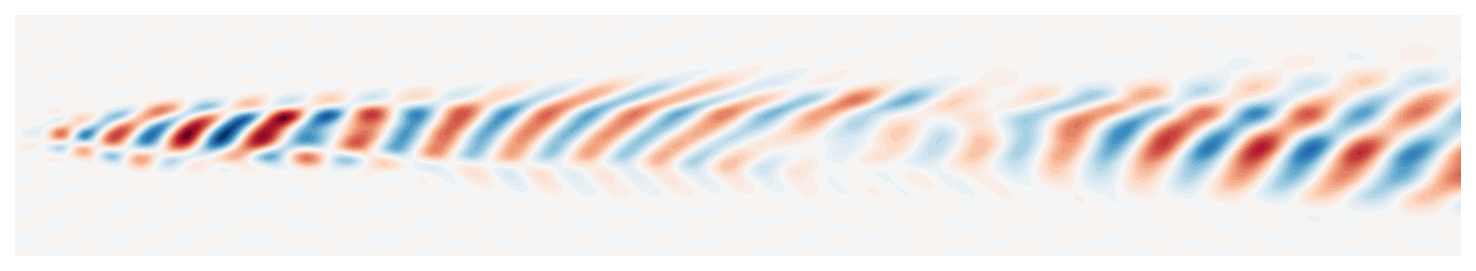
\includegraphics[width=\linewidth]{IMAGES/DMD_MODES_main_freqs_T1200/DMD_mode_St0.84.png}
        \caption{Mode at $St = 0.84$}
        \label{fig:modes_1200K_2}
    \end{subfigure}
    \\[1em]
    \begin{subfigure}[b]{0.48\textwidth}
        \centering
        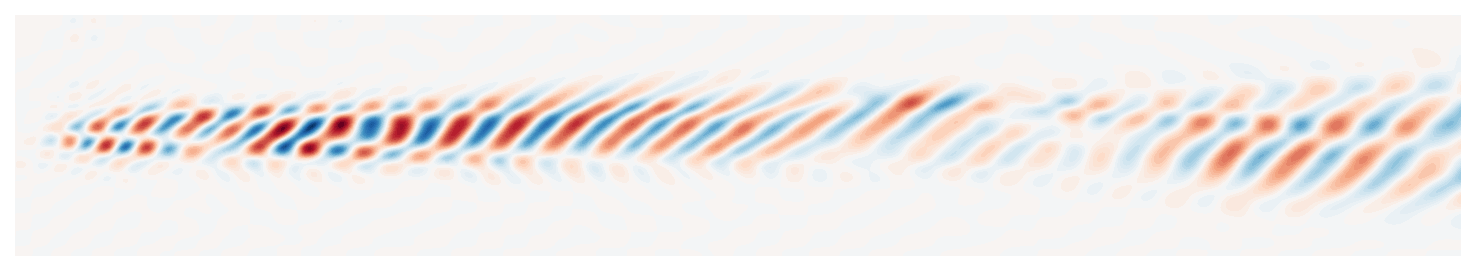
\includegraphics[width=\linewidth]{IMAGES/DMD_MODES_main_freqs_T1200/DMD_mode_St1.26.png}
        \caption{Mode at $St = 1.26$}
        \label{fig:modes_1200K_3}
    \end{subfigure}
    \hfill
    \begin{subfigure}[b]{0.48\textwidth}
        \centering
        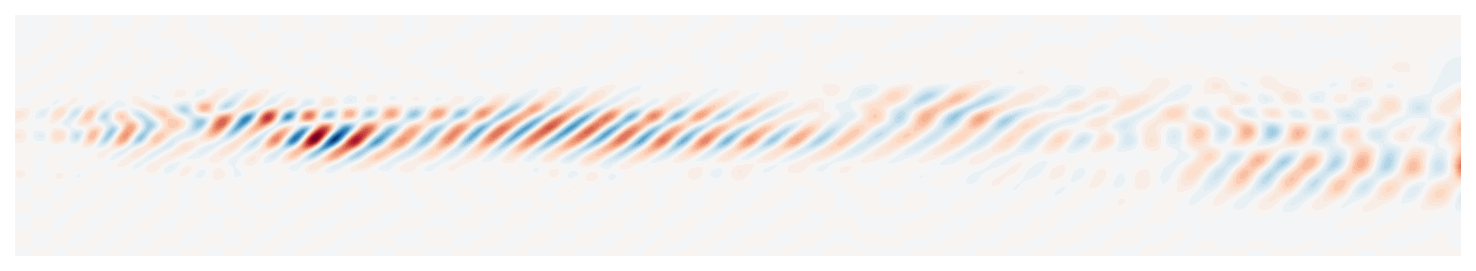
\includegraphics[width=\linewidth]{IMAGES/DMD_MODES_main_freqs_T1200/DMD_mode_St1.68.png}
        \caption{Mode at $St = 1.68$}
        \label{fig:modes_1200K_4}
    \end{subfigure}
    \caption{DMD temperature modes for the 1200~K dataset at the main harmonic frequencies ($St = 0.42$, $0.84$, $1.26$, $1.68$), corresponding to $f$, $2f$, $3f$, and $4f$ respectively.}
    \label{fig:modes_1200K}
\end{figure}
\FloatBarrier

\paragraph{Case 1500~K}
\label{sec:spectrum_1500K}

The 1500~K spectrum, shown in Figure~\ref{fig:spectrum_1500K_combination}, exhibits a structure closely analogous to the 1200~K case, with the dominant peak again located at $St \approx 0.42$. Secondary peaks are found at $St \approx 0.81$, $St \approx 1.22$, and $St \approx 1.47$.  In this case however, the spectrum shows other spectral peaks as highlighted in Figure~\ref{fig:spectrum_1500K_combination} in green. These peaks rapresent the interaction between main frequencies typical of the quasi periodic regime.
\FloatBarrier
\begin{figure}[h!]
    \centering
    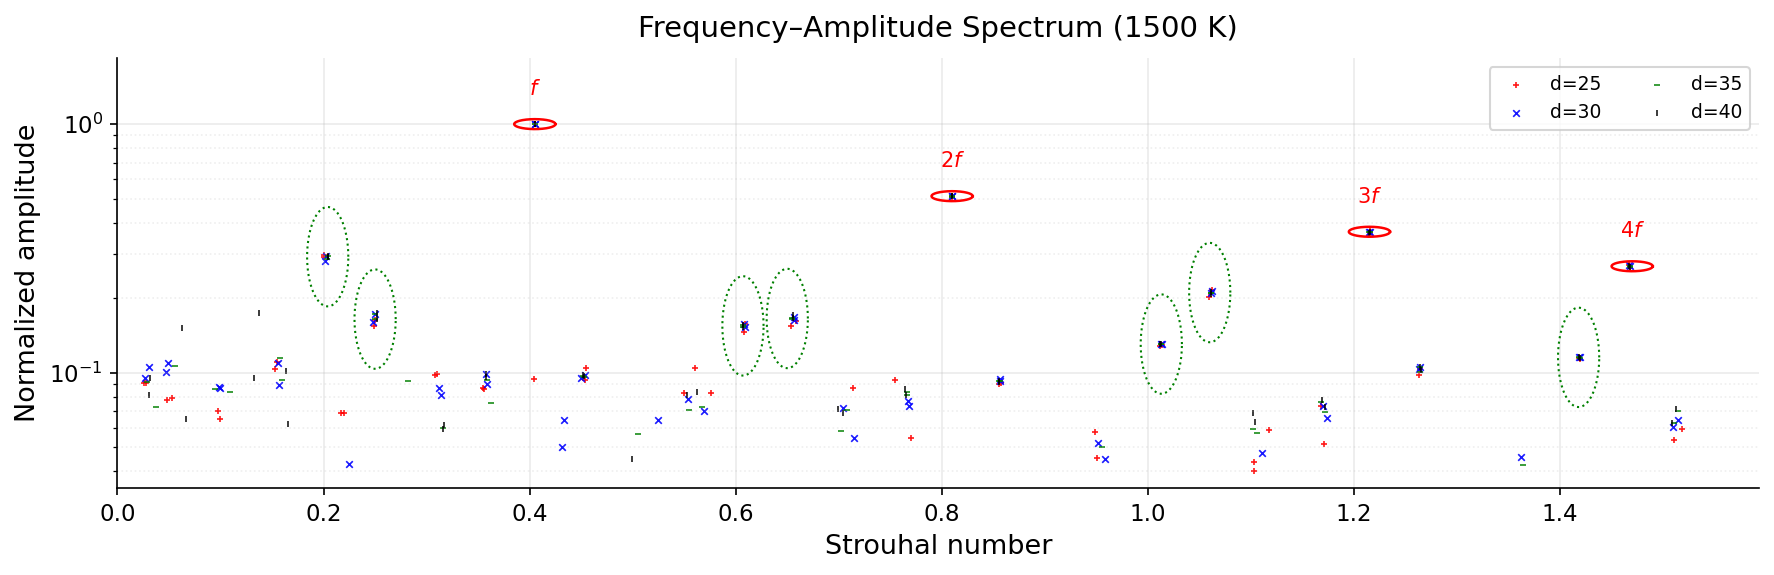
\includegraphics[width=\textwidth]{IMAGES/Spectrum_1500K_d25_30_35_40_tol4e-02_5e-02.png}
    \caption{Normalised DMD mode amplitudes as a function of Strouhal number for the 1500~K dataset, for $d \in \{35,40,45\}$ and $\varepsilon_{\mathrm{tol}} \in \{5\times10^{-2},\, 7\times10^{-2}\}$. Red solid ellipses mark the main harmonic series ($f$, $2f$, $3f$); green dashed ellipses mark the quasi-periodic combination tones.}
    \label{fig:spectrum_1500K_combination}
\end{figure}
\FloatBarrier

The associated modes to the main harmonic frequencies circled in red in Figure~\ref{fig:spectrum_1500K_combination} are shown in Figure~\ref{fig:modes_1500K}.

\FloatBarrier
\begin{figure}[h!]
    \centering
    \begin{subfigure}[b]{0.48\textwidth}
        \centering
        
\includegraphics[width=\linewidth]{IMAGES/DMD_MODES_main_freqs_T1500/DMD_mode_St0.41.png}
        \caption{Mode at $St = 0.41$}
        \label{fig:modes_1500K_1}
    \end{subfigure}
    \hfill
    \begin{subfigure}[b]{0.48\textwidth}
        \centering
        
\includegraphics[width=\linewidth]{IMAGES/DMD_MODES_main_freqs_T1500/DMD_mode_St0.81.png}
        \caption{Mode at $St = 0.81$}
        \label{fig:modes_1500K_2}
    \end{subfigure}
    \\[1em]
    \begin{subfigure}[b]{0.48\textwidth}
        \centering
        
\includegraphics[width=\linewidth]{IMAGES/DMD_MODES_main_freqs_T1500/DMD_mode_St1.22.png}
        \caption{Mode at $St = 1.22$}
        \label{fig:modes_1500K_3}
    \end{subfigure}
    \hfill
    \begin{subfigure}[b]{0.48\textwidth}
        \centering
        
\includegraphics[width=\linewidth]{IMAGES/DMD_MODES_main_freqs_T1500/DMD_mode_St1.47.png}
        \caption{Mode at $St = 1.47$}
        \label{fig:modes_1500K_4}
    \end{subfigure}
    \caption{DMD temperature modes for the 1500~K dataset at the main harmonic frequencies ($St = 0.41$, $0.81$, $1.22$, $1.47$), corresponding to $f$, $2f$, $3f$, and $4f$ respectively.}
    \label{fig:modes_1500K}
\end{figure}
\FloatBarrier

Figure~\ref{fig:comb_modes_1500K} shows the modes associated to the quasi-periodic combination frequencies highlighted in green in Figure~\ref{fig:spectrum_1500K_combination}.
\FloatBarrier
\begin{figure}[h!]
    \centering
    \begin{subfigure}[b]{0.48\textwidth}
        \centering
        
\includegraphics[width=\linewidth]{IMAGES/DMD_MODES_main_freqs_T1500/DMD_mode_St0.20.png}
        \caption{Mode at $St = 0.20$}
        \label{fig:comb_modes_1500K_1}
    \end{subfigure}
    \hfill
    \begin{subfigure}[b]{0.48\textwidth}
        \centering
        
\includegraphics[width=\linewidth]{IMAGES/DMD_MODES_main_freqs_T1500/DMD_mode_St0.61.png}
        \caption{Mode at $St = 0.61$}
        \label{fig:comb_modes_1500K_2}
    \end{subfigure}
    \\[1em]
    \begin{subfigure}[b]{0.48\textwidth}
        \centering
        
\includegraphics[width=\linewidth]{IMAGES/DMD_MODES_main_freqs_T1500/DMD_mode_St1.01.png}
        \caption{Mode at $St = 1.01$}
        \label{fig:comb_modes_1500K_3}
    \end{subfigure}
    \hfill
    \begin{subfigure}[b]{0.48\textwidth}
        \centering
        
\includegraphics[width=\linewidth]{IMAGES/DMD_MODES_main_freqs_T1500/DMD_mode_St1.42.png}
        \caption{Mode at $St = 1.42$}
        \label{fig:comb_modes_1500K_4}
    \end{subfigure}
    \caption{DMD temperature modes for the 1500~K dataset at the quasi-periodic combination frequencies ($St = 0.20$, $0.61$, $1.01$, $1.42$), highlighted by green ellipses in Figure~\ref{fig:spectrum_1500K_combination}.}
    \label{fig:comb_modes_1500K}
\end{figure}
\FloatBarrier

\paragraph{Case 1700~K}
\label{sec:spectrum_1700K}

The 1700~K case, shown in Figure~\ref{fig:spectrum_1700K}, presents a different spectral structure. The dominant peak remains at $St \approx 0.40$, consistent with the lower-temperature cases, but the overall spectrum is sparser: maximum relevant Strouhal number observed is $St \approx 1.25$ and fewer secondary modes are retained. In addition to the main harmonic series, two low-frequency peaks at $St \approx 0.11$ and $St \approx 0.19$, highlighted in blue in Figure~\ref{fig:spectrum_1700K}, are identified across multiple parameter combinations.

\FloatBarrier
\begin{figure}[h!]
    \centering
    
\includegraphics[width=\textwidth]{Frequency_amplitude_plot1700.png}
    \caption{Normalised DMD mode amplitudes as a function of Strouhal number for the 1700~K dataset, for $d \in \{35,40,45\}$ and $\varepsilon_{\mathrm{tol}} \in \{5\times10^{-2},\, 7\times10^{-2}\}$.}
    \label{fig:spectrum_1700K}
\end{figure}
\FloatBarrier

The associated modes to the highlighted points in Figure~\ref{fig:spectrum_1700K} are shown in Figure~\ref{fig:modes_1700K}.

\FloatBarrier
\begin{figure}[h!]
    \centering
    \begin{subfigure}[b]{0.32\textwidth}
        \centering
        
\includegraphics[width=\linewidth]{IMAGES/DMD_MODES_main_freqs_T1700/DMD_mode_St0.41.png}
        \caption{Mode at $St = 0.41$}
        \label{fig:modes_1700K_1}
    \end{subfigure}
    \hfill
    \begin{subfigure}[b]{0.32\textwidth}
        \centering
        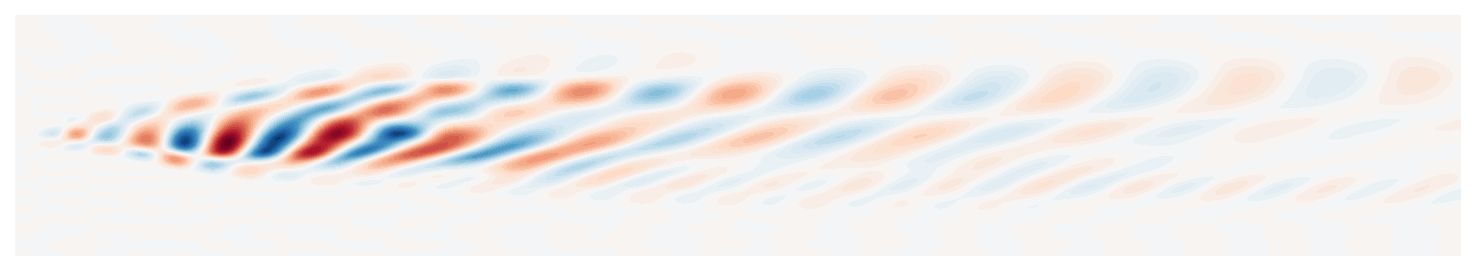
\includegraphics[width=\linewidth]{IMAGES/DMD_MODES_main_freqs_T1700/DMD_mode_St0.82.png}
        \caption{Mode at $St = 0.82$}
        \label{fig:modes_1700K_2}
    \end{subfigure}
    \hfill
    \begin{subfigure}[b]{0.32\textwidth}
        \centering
        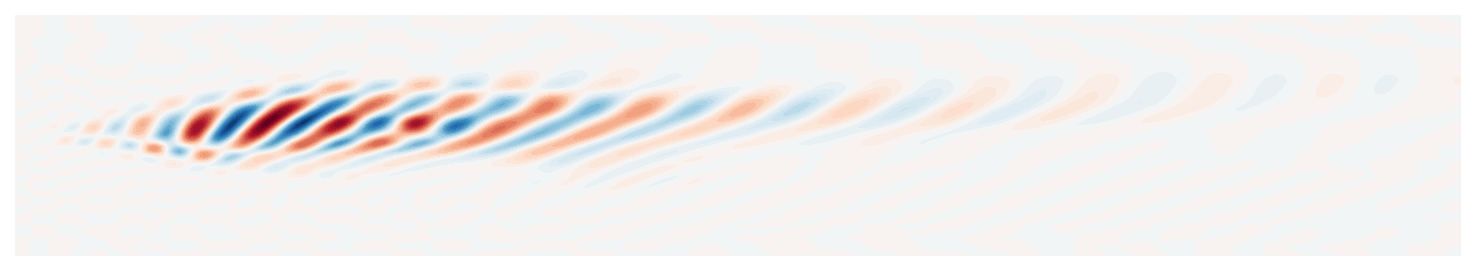
\includegraphics[width=\linewidth]{IMAGES/DMD_MODES_main_freqs_T1700/DMD_mode_St1.23.png}
        \caption{Mode at $St = 1.23$}
        \label{fig:modes_1700K_3}
    \end{subfigure}
    \\[1em]
    \begin{subfigure}[b]{0.48\textwidth}
        \centering
        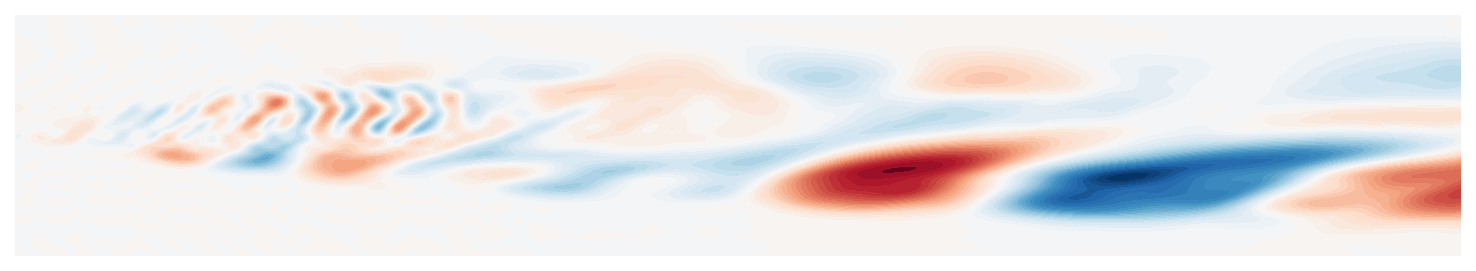
\includegraphics[width=\linewidth]{IMAGES/DMD_MODES_main_freqs_T1700/DMD_mode_St0.11.png}
        \caption{Mode at $St = 0.11$}
        \label{fig:modes_1700K_4}
    \end{subfigure}
    \hfill
    \begin{subfigure}[b]{0.48\textwidth}
        \centering
        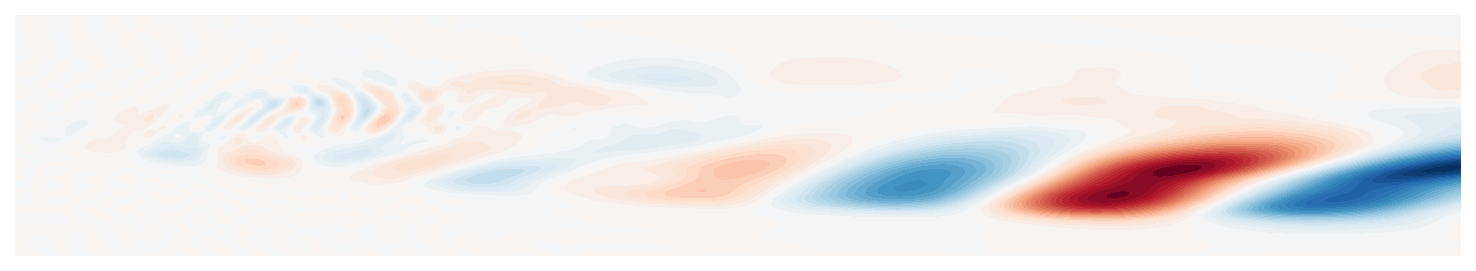
\includegraphics[width=\linewidth]{IMAGES/DMD_MODES_main_freqs_T1700/DMD_mode_St0.19.png}
        \caption{Mode at $St = 0.19$}
        \label{fig:modes_1700K_5}
    \end{subfigure}
    \caption{DMD temperature modes for the 1700~K dataset. Top row: modes at the three main harmonic frequencies ($St = 0.41,\,0.82,\,1.23$). Bottom row: modes at the additional frequencies highlighted in blue in Figure~\ref{fig:spectrum_1700K} ($St = 0.11,\,0.19$).}
    \label{fig:modes_1700K}
\end{figure}
\FloatBarrier

\subsubsection*{Discussion: Spectral and Spatial Evolution Across Preheat Temperatures}

The main focus of this analysis was that of understanding how flow changes in the three cases, rather than investigating the difference in chemical behaviour. Despite this, in practical cases these regimes yield different efficiency-poolutants tradoff, with the lowest temperature case beeing the least efficient and least polluting one and the higher temperature case to have the highest $NO_x$ emission levels and most mixing.

The first case analyzed, i.e. 1200~K has an harmonic flow with with a dominant peak at $St \approx 0.42$ is accompanied by secondary peaks at approximately integer multiples of this frequency extending up to $St \approx 1.7$. This is the sign of a strongly periodic shear layer instability, and the modes reported in Figure~\ref{fig:modes_1200K} show that the phenomenon develops in the far field. This is reflects downstream convection and roll-up of large-scale vortices that have had space and time to develop along the mixing layer.

On the other hand, at 1700~K, the spectral picture changes substantially. While the dominant frequency is preserved at $St \approx 0.40$, confirming that the primary instability mechanism remains kinematically controlled by the shear between the two inlet streams, the harmonic content is severly reduced, and the overall spectrum is sparser. By observing the modes reported in Figure~\ref{fig:modes_1700K}, one can see that the main instability develops in the near field. This can be explained by the fact that the stronger heat release ties the energetically significant dynamics to the  attachment point.

The 1500~K case contains the transition between the two cases. This is particularly relevant from a physical point of view due to the fact that is a balance between the two regimes. In turn this means that understanding the flow structure might help in designing more efficient combustion processes that suppress $NO_x$ formation.
In this spectrum we can find dominant harmonic structures as in the 1200~K, but additionally the creation of quasi-periodic frequencies highlighted in green in Figure~\ref{fig:spectrum_1500K_combination}. This quasi-periodic spectral content can be interpreted as a signature of the competing dynamics active at this operating point: the primary shear-layer instability is still present, but thermal effects are beginning to modify the nonlinear interactions.
The transient case, i.e. 1500~K has energetically significant DMD modes in both the far field and the near field regions as shown in Figures~\ref{fig:modes_1500K} and \ref{fig:comb_modes_1500K}. In this regime the instabilities are affected by both the far field convective instability and the energy release near the inlet.

To sum up, the analysis shows that increasing preheat temperature shifts the flow dynamics to the near field and supports a transition from a harmonic (periodic) regime to a less harmonic, more complex/quasi-periodic regime.
 Further investigation along this research direction, extending the modal analysis to additional operating conditions and coupling it with chemical kinetics data is required to provide better characterization of pollutant formation for the flow.
